\documentclass[11pt]{article}
\usepackage[margin=1in]{geometry}
\usepackage{amsmath,amssymb,amsthm,mathtools}
\usepackage{booktabs}
\usepackage{enumitem}
\usepackage{hyperref}
\usepackage{tikz}
\usetikzlibrary{arrows.meta,calc,fit,positioning,shapes.geometric}

\newcommand{\Worldline}{\ensuremath{\mathsf{Worldline}}}
\newcommand{\Strand}{\ensuremath{\mathsf{Strand}}}
\newcommand{\Braid}{\ensuremath{\mathsf{Braid}}}
\newcommand{\View}{\ensuremath{\mathsf{View}}}
\newcommand{\Conflict}{\ensuremath{\mathsf{Conflict}}}
\newcommand{\Witness}{\ensuremath{\mathsf{Witness}}}
\newcommand{\Lower}{\ensuremath{\mathsf{Lower}}}
\newcommand{\Merge}{\ensuremath{\mathsf{Merge}}}
\newcommand{\Lift}{\ensuremath{\mathsf{Lift}}}
\newcommand{\Replay}{\ensuremath{\mathsf{Replay}}}
\newcommand{\State}{\ensuremath{\mathsf{State}}}
\newcommand{\Proj}{\pi}

\theoremstyle{definition}
\newtheorem{definition}{Definition}
\newtheorem{observation}{Observation}
\newtheorem{principle}{Principle}
\newtheorem{proposition}{Proposition}
\newtheorem{example}{Example}

\title{Causal Lifting and Merge Conflicts\\[6pt]
\large What Higher-Dimensional Merge Can Eliminate, and What It Cannot\\[3pt]
\normalsize 2026-04-09}
\author{}
\date{}

\begin{document}
\maketitle

\section{Purpose}

This note sharpens one tempting but dangerous intuition:

\begin{quote}
``Merge conflicts happen because the merge is happening through a lossy
projection. If we lift the merge into a richer space and carry enough witness,
maybe we can eliminate merge conflicts.''
\end{quote}

That intuition is \emph{good}, but only after it is separated into three
claims:
\begin{enumerate}[leftmargin=2em]
\item many merge conflicts \emph{are} artifacts of lossy lowering,
\item a richer causal merge can eliminate many of those spurious conflicts,
\item no amount of lifting removes \emph{genuine} semantic or governance
  incompatibility.
\end{enumerate}

The point of this note is to separate what is real from what is wishful
thinking, using the current WARP / Observer Geometry / optics vocabulary.

\section{Short Answer}

\begin{principle}[The right sharpened thesis]
The stack should not promise ``no merge conflicts ever.'' It should promise
something stronger and more honest:
\begin{enumerate}[leftmargin=2em]
\item eliminate conflicts caused only by lossy projection,
\item preserve genuine incompatibility as explicit causal structure rather than
  flattening it into opaque failure,
\item carry enough witness to lower merged causal structure back into an
  observer-relative surface lawfully.
\end{enumerate}
\end{principle}

\begin{observation}[The dream is not nonsense]
The useful dream is \emph{not} that higher-dimensional merge magically makes
all edits compatible. The useful dream is that many apparent conflicts are not
real semantic conflicts at all; they are artifacts of trying to merge after
too much structure has already been forgotten.
\end{observation}

\section{Why Ordinary Merge So Often Feels Wrong}

A plain text merge usually operates on a representation that has already thrown
away some or all of the following:
\begin{itemize}[leftmargin=2em]
\item causal history,
\item author intent,
\item rewrite footprint,
\item structural identity,
\item local witness needed for lawful reassembly.
\end{itemize}

At that point the merge engine sees only the lowered surface:
\[
\Lower : \text{richer causal object} \to \text{flattened artifact}.
\]

If the lowering is lossy, then independence in the richer space may become
aliasing in the lowered space. Two edits that are causally disjoint can project
to the same line, the same token span, or the same serialized order slot.

\begin{figure}[h]
\centering
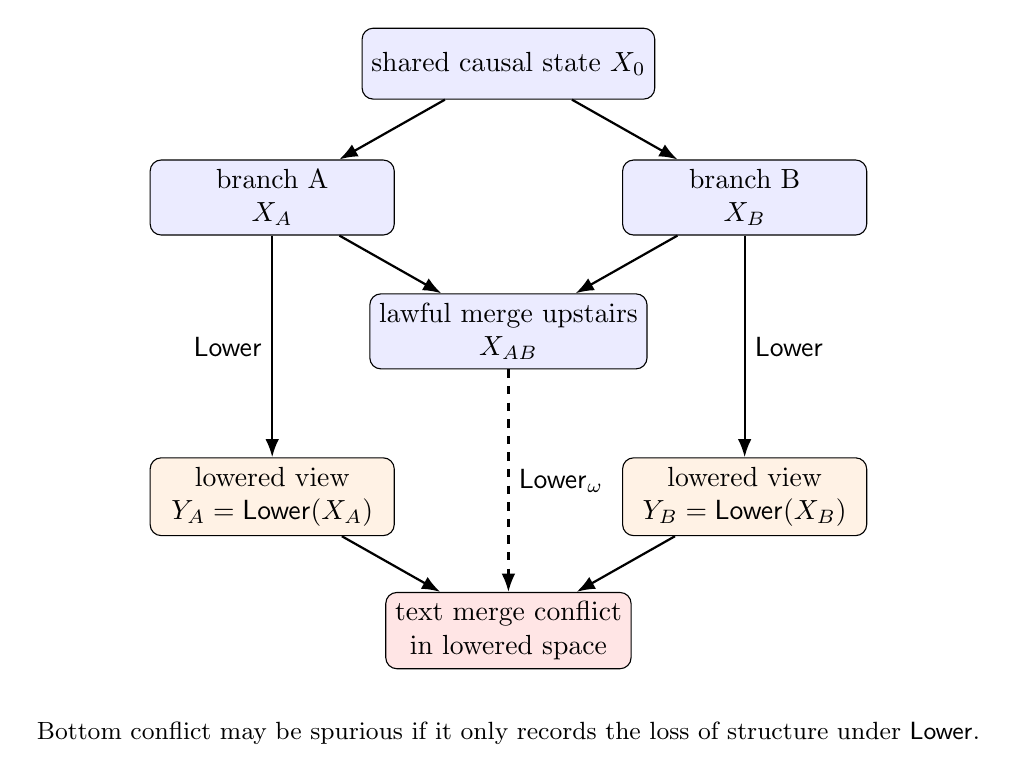
\begin{tikzpicture}[
  box/.style={draw, rounded corners, minimum width=3.1cm, minimum height=0.9cm, align=center},
  rich/.style={box, fill=blue!8},
  poor/.style={box, fill=orange!10},
  bad/.style={box, fill=red!10},
  arr/.style={-Latex, thick}
]
\node[rich] (x0) at (0,4) {shared causal state $X_0$};
\node[rich] (x1) at (-3,2.3) {branch A\\$X_A$};
\node[rich] (x2) at (3,2.3) {branch B\\$X_B$};
\node[rich] (xm) at (0,0.6) {lawful merge upstairs\\$X_{AB}$};

\node[poor] (y1) at (-3,-1.5) {lowered view\\$Y_A = \Lower(X_A)$};
\node[poor] (y2) at (3,-1.5) {lowered view\\$Y_B = \Lower(X_B)$};
\node[bad] (yc) at (0,-3.2) {text merge conflict\\in lowered space};

\draw[arr] (x0) -- (x1);
\draw[arr] (x0) -- (x2);
\draw[arr] (x1) -- (xm);
\draw[arr] (x2) -- (xm);

\draw[arr] (x1) -- node[left] {$\Lower$} (y1);
\draw[arr] (x2) -- node[right] {$\Lower$} (y2);
\draw[arr,dashed] (xm) -- node[right] {$\Lower_\omega$} (yc);
\draw[arr] (y1) -- (yc);
\draw[arr] (y2) -- (yc);

\node[align=center] at (0,-4.5) {\small Bottom conflict may be spurious if it only records the loss of structure under $\Lower$.};
\end{tikzpicture}
\caption{A conflict can appear after lowering even when a lawful merge exists in richer causal space.}
\end{figure}

\section{The Three Useful Distinctions}

\subsection{1. Projection Conflicts}

These are conflicts caused by the lowering surface rather than by the domain.
Two edits are compatible in the richer space, but the chosen serialization or
observer projection makes them look incompatible.

\begin{example}[Projection conflict]
Two writers independently add different keys to the same logical map:
\begin{align*}
\text{Base} \quad & \{\texttt{flags}: \{\}\} \\
\text{Branch A} \quad & \{\texttt{flags}: \{\texttt{admin}: \texttt{true}\}\} \\
\text{Branch B} \quad & \{\texttt{flags}: \{\texttt{beta}: \texttt{true}\}\}
\end{align*}

If the file is stored on one line, a line-based merge may conflict even though
the logical map merge is trivial:
\[
\{\texttt{admin}: \texttt{true},\ \texttt{beta}: \texttt{true}\}.
\]

The conflict is real in the lowered text surface, but not in the richer
structured state.
\end{example}

\subsection{2. Semantic Conflicts}

These are genuine incompatibilities in the domain itself. They survive lifting.

\begin{example}[Semantic conflict]
Suppose a graph stores a singleton field:
\[
\texttt{primaryColor} \in \{\texttt{red},\texttt{green},\texttt{blue}\}.
\]

Branch A sets
\[
\texttt{primaryColor} := \texttt{red}
\]
while Branch B sets
\[
\texttt{primaryColor} := \texttt{green}.
\]

No richer merge space can honestly claim these are the same canonical state.
The system may:
\begin{itemize}[leftmargin=2em]
\item preserve both intents in a conflict object,
\item fork into strands,
\item apply a governance policy,
\item or ask a human / agent / policy layer to choose.
\end{itemize}

But this is not a projection artifact. It is a genuine incompatibility.
\end{example}

\subsection{3. Governance Conflicts}

Sometimes both alternatives are valid but the system still needs a choice.
These conflicts are not about impossibility; they are about authority, policy,
or social contract.

\begin{example}[Governance conflict]
Two release branches each update the ``release notes headline'' to a different
marketing message. Both are coherent edits. The problem is not semantics of
graph composition; the problem is that the product surface wants one final
headline.
\end{example}

\section{The Optic View}

The current working WARP optic shape is:
\[
\Omega = (\Proj,\mathcal{F},\rho,\omega,\sigma)
\]
where:
\begin{itemize}[leftmargin=2em]
\item $\Proj$ is an observer-relative projection,
\item $\mathcal{F}$ is the footprint / focus boundary,
\item $\rho$ is the local rewrite,
\item $\omega$ is the witness sufficient for lawful reassembly or inversion,
\item $\sigma$ is reintegration into the updated whole.
\end{itemize}

This gives a clean way to think about merge:
\begin{enumerate}[leftmargin=2em]
\item lift edits into optic-bearing causal objects,
\item compare footprints and witnesses,
\item compose where lawful,
\item record explicit obstruction where composition fails,
\item lower back into an observer-relative surface with enough witness to make
  that lowering lawful.
\end{enumerate}

\begin{observation}[Conflict as obstruction]
In this frame, a conflict is not first an exception string. It is first an
obstruction to optic composition. The conflict artifact is the witness of that
obstruction.
\end{observation}

\begin{figure}[h]
\centering
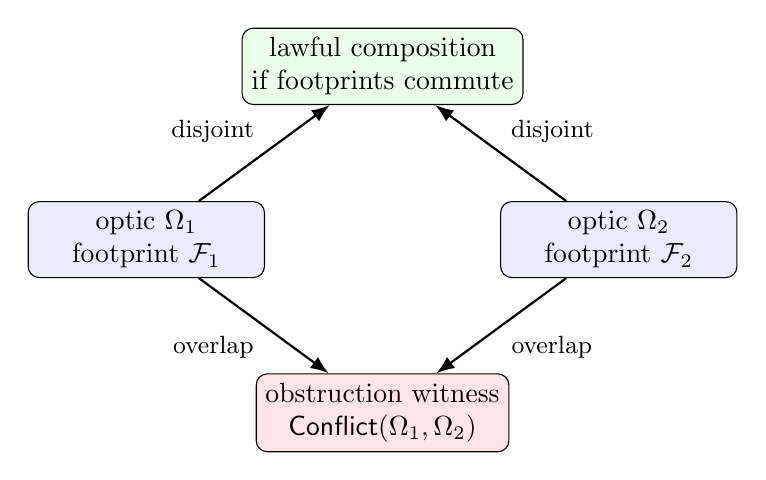
\begin{tikzpicture}[
  box/.style={draw, rounded corners, minimum width=3.0cm, minimum height=0.9cm, align=center},
  a/.style={box, fill=blue!8},
  b/.style={box, fill=green!8},
  c/.style={box, fill=red!10},
  arr/.style={-Latex, thick}
]
\node[a] (o1) at (-3,0) {optic $\Omega_1$\\footprint $\mathcal{F}_1$};
\node[a] (o2) at (3,0) {optic $\Omega_2$\\footprint $\mathcal{F}_2$};
\node[c] (obs) at (0,-2.2) {obstruction witness\\$\Conflict(\Omega_1,\Omega_2)$};
\node[b] (ok) at (0,2.2) {lawful composition\\if footprints commute};

\draw[arr] (o1) -- node[above left] {\small disjoint} (ok);
\draw[arr] (o2) -- node[above right] {\small disjoint} (ok);

\draw[arr] (o1) -- node[below left] {\small overlap} (obs);
\draw[arr] (o2) -- node[below right] {\small overlap} (obs);
\end{tikzpicture}
\caption{Disjoint optics compose; overlapping optics may produce an explicit obstruction witness.}
\end{figure}

\section{What Lifting Can Actually Buy}

\begin{proposition}[Causal lifting removes spurious conflicts]
If two rewrites are independent in the richer causal space and the lowering
surface aliases them only because it forgot the distinctions proving that
independence, then merging before lowering can eliminate the apparent conflict.
\end{proposition}

\noindent This is the main positive result you are intuiting.

\begin{example}[Import conflict that disappears upstairs]
Suppose two branches edit a source file:
\begin{itemize}[leftmargin=2em]
\item Branch A adds an import and uses it in a new helper.
\item Branch B reorders or reformats the import block while touching the same
  line region.
\end{itemize}

At the plain text level:
\begin{itemize}[leftmargin=2em]
\item the import block may conflict,
\item the formatter output may alias both edits to the same lines.
\end{itemize}

At the richer structured level:
\begin{itemize}[leftmargin=2em]
\item the imported symbol identity is explicit,
\item the helper insertion has its own structural location,
\item import normalization can be deferred to lowering.
\end{itemize}

So the conflict is not ``these edits are incompatible.'' It is
``the lowered textual surface is too poor to show their independence.''
\end{example}

\begin{proposition}[Lifting does not remove genuine incompatibility]
If two rewrites demand incompatible values for the same invariant-bearing slot,
or require mutually exclusive reintegrations, then no amount of lifting can
honestly identify them as one canonical state.
\end{proposition}

\begin{example}[Two moves into different parents]
A node in a tree can have one parent. Branch A moves the node under
\texttt{Menu/Header}. Branch B moves the same node under
\texttt{Menu/Footer}. A richer merge space can preserve both intents, compute
distance between them, and keep witness of each move. But unless the domain has
a lawful ``both'' interpretation, this remains a genuine incompatibility.
\end{example}

\section{The Role of Witness in Lowering}

The user intuition about ``a witness for lowering it back'' is especially good.
That is the crucial extra piece.

Without witness, a rich merge may still leave you with a problem:
\begin{quote}
``I know the merged causal structure, but I do not know how to produce the
lowered artifact lawfully or stably.''
\end{quote}

The witness is what tells the system enough about:
\begin{itemize}[leftmargin=2em]
\item identity,
\item attachment points,
\item residual context,
\item inversion,
\item and lawful reassembly
\end{itemize}
to lower the merged structure without guessing.

\begin{figure}[h]
\centering
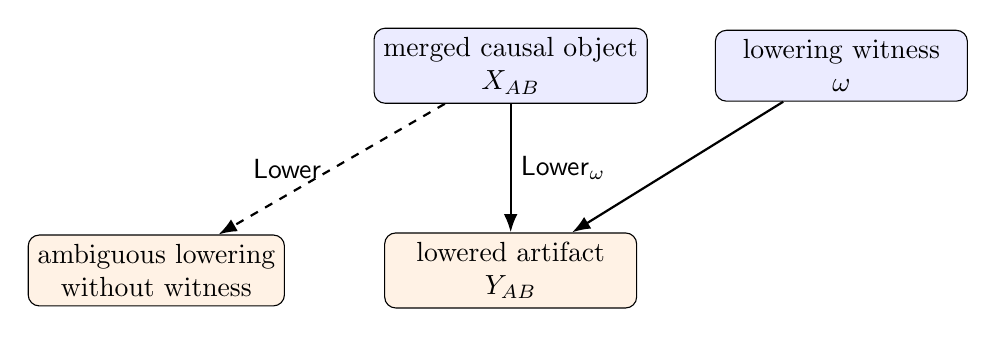
\begin{tikzpicture}[
  box/.style={draw, rounded corners, minimum width=3.2cm, minimum height=0.9cm, align=center},
  top/.style={box, fill=blue!8},
  low/.style={box, fill=orange!10},
  arr/.style={-Latex, thick}
]
\node[top] (merge) at (0,2.6) {merged causal object\\$X_{AB}$};
\node[top] (wit) at (4.2,2.6) {lowering witness\\$\omega$};
\node[low] (surface) at (0,0) {lowered artifact\\$Y_{AB}$};
\node[low] (bad) at (-4.5,0) {ambiguous lowering\\without witness};

\draw[arr] (merge) -- node[right] {$\Lower_\omega$} (surface);
\draw[arr] (wit) -- (surface);
\draw[arr,dashed] (merge) -- node[left] {$\Lower$} (bad);
\end{tikzpicture}
\caption{Witness separates lawful lowering from ambiguous reserialization.}
\end{figure}

\begin{observation}[Lowering choice is not always conflict]
Even after a clean causal merge, the lowered artifact may still require
presentation choices:
\begin{itemize}[leftmargin=2em]
\item ordering,
\item formatting,
\item canonical pretty-printing,
\item or observer-relative redaction.
\end{itemize}

These should not be confused with semantic conflicts. They are lowering policy
questions.
\end{observation}

\section{Where Strands and Braids Help}

Strands and braids make the picture more honest.

\begin{itemize}[leftmargin=2em]
\item A \Strand{} preserves one speculative causal lane.
\item A \Braid{} is a composite read over multiple lanes.
\end{itemize}

This means the system does not have to pretend that one immediate canonical
state always exists. It can:
\begin{enumerate}[leftmargin=2em]
\item keep both speculative lanes alive,
\item read them together in a braid,
\item compute conflict / distance / witness data over the pair,
\item later collapse only the relevant causal slice into canonical history.
\end{enumerate}

\begin{figure}[h]
\centering
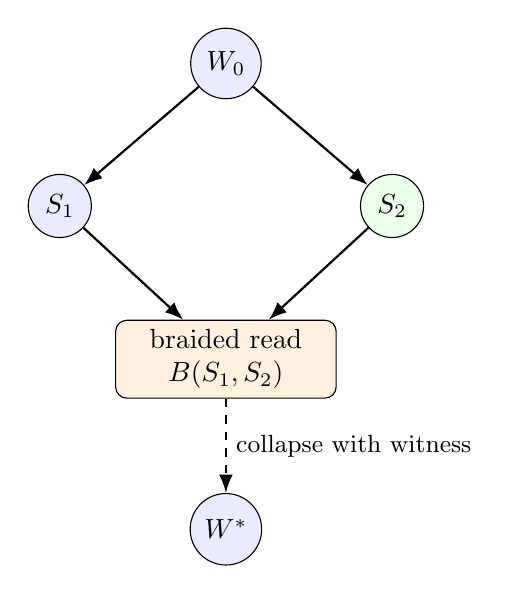
\begin{tikzpicture}[
  node distance=1.2cm and 1.5cm,
  state/.style={draw, circle, minimum size=0.75cm, fill=blue!8},
  strand/.style={draw, circle, minimum size=0.75cm, fill=green!8},
  braid/.style={draw, rounded corners, fill=orange!12, minimum width=2.8cm, minimum height=0.9cm, align=center},
  arr/.style={-Latex, thick}
]
\node[state] (w0) {$W_0$};
\node[state, below left=of w0] (s1) {$S_1$};
\node[strand, below right=of w0] (s2) {$S_2$};
\node[braid, below=2.8cm of w0] (b) {braided read\\$B(S_1,S_2)$};
\node[state, below=5cm of w0] (c) {$W^\ast$};

\draw[arr] (w0) -- (s1);
\draw[arr] (w0) -- (s2);
\draw[arr] (s1) -- (b);
\draw[arr] (s2) -- (b);
\draw[arr,dashed] (b) -- node[right] {\small collapse with witness} (c);
\end{tikzpicture}
\caption{Strands preserve alternatives; braids permit structured joint reading before any final collapse.}
\end{figure}

\begin{observation}[Braids do not erase conflict]
Braiding is not magic. It does not make incompatible intents suddenly
compatible. What it does is preserve both causal lanes without prematurely
destroying information.
\end{observation}

\section{A Practical Classification Table}

\begin{center}
\begin{tabular}{@{}p{3.2cm}p{3.7cm}p{3.0cm}p{3.2cm}@{}}
\toprule
Case & What is really happening & Can lifting help? & Best outcome \\
\midrule
Formatting / ordering clash & Lowered surface aliases independent edits & Yes, often completely & Merge upstairs, lower with canonical formatting witness \\
\addlinespace
Structural alias clash & Two edits hit same text span but different graph/AST identities & Yes, often strongly & Merge on structure, not text \\
\addlinespace
Singleton invariant clash & Both edits claim incompatible canonical truth & No, not as one state & Preserve explicit conflict or keep parallel strands \\
\addlinespace
Policy / authority clash & Both edits are valid but one public surface must choose & Only partially & Preserve alternatives, then resolve by governance policy \\
\bottomrule
\end{tabular}
\end{center}

\section{What Is Real, and What Is Overreach}

\subsection{Real}

These claims are strong and defensible:
\begin{itemize}[leftmargin=2em]
\item Many merge conflicts are artifacts of merging after lossy lowering.
\item Merge should happen on a richer causal object whenever possible.
\item The witness is what makes lawful lowering and inversion possible.
\item Genuine incompatibility should be represented as explicit causal data,
  not flattened into stringly merge junk.
\item Strands and braids let the system preserve alternatives rather than
  forcing premature canonical collapse.
\end{itemize}

\subsection{Overreach}

These claims are too strong:
\begin{itemize}[leftmargin=2em]
\item ``There is always some higher-dimensional merge that removes the
  conflict.''
\item ``Enough math means no conflicts at all.''
\item ``Any disagreement is evidence of a bad projection.''
\end{itemize}

Sometimes the edits really do disagree.

\section{The Best One-Sentence Version}

If you want one sentence that keeps the dream but avoids nonsense, use this:

\begin{quote}
\emph{WARP should not merely auto-resolve merge conflicts; it should lift
merge into causal space so that spurious conflicts disappear, while genuine
incompatibilities survive as explicit witnessed obstructions rather than lossy
text failures.}
\end{quote}

\section{A Study Exercise}

When you encounter a merge conflict, ask these questions in order:
\begin{enumerate}[leftmargin=2em]
\item What distinctions did the lowered surface forget?
\item If I restore causal identity, do the edits still interfere?
\item Are their footprints actually overlapping?
\item If they overlap, is the overlap semantically incompatible or merely
  representationally awkward?
\item If they remain incompatible, is the issue semantic or governance?
\item What witness would I need to lower the merged result back lawfully?
\end{enumerate}

That exercise will train the right instinct very quickly.

\section{One-Sentence Summary}

The useful mathematical dream is not the abolition of all conflict; it is the
replacement of lossy, projection-induced conflicts by causal merge with witness,
plus explicit first-class obstruction objects for the incompatibilities that are
actually real.

\end{document}
